\documentclass[12pt,letterpaper]{article}
\usepackage{amsmath}
\usepackage{amsfonts}
%\usepackage{color}
\usepackage[usenames,dvipsnames]{color}
\usepackage{graphicx}
\usepackage{longtable}
\usepackage{rotating}
\usepackage{verbatim}
\usepackage[pdftex,bookmarksopen]{hyperref}
\hypersetup{pdfauthor={John Sibert}}
\hypersetup{pdfsubject={Compartment model of MHI YFT}}
\hypersetup{pdftitle={Two-compartment models of Main Hawaiian Islands
Yellowfin Tuna Population}}
\hypersetup{pdfkeywords={yellowfin,state space,compartment model,Hawaii}}

\newcommand\doublespacing{\baselineskip=1.6\normalbaselineskip}
\newcommand\singlespacing{\baselineskip=1.0\normalbaselineskip}
\renewcommand\deg[1]{$^\circ$#1}
\newcommand\SD{SEAPODYM}
\newcommand\MFCL{MULTIFAN-CL}
\newcommand\ADMB{ADModel Builder}
\newcommand\SPC{Secretariat of the Pacific Community}
\newcommand\WCPO{Western Central Pacific Ocean}
\newcommand\SSAP{Skipjack Survey and Assessment Programme}
\newcommand\RTTP{Regional Tuna Tagging Programme}
\newcommand\PTTP{Pacific Tuna Tagging Programme}
\newcommand\FAD{fish aggregating device}
\newcommand\ADRM{advection-diffusion-reaction model}
\newcommand\help[1]{\color{Magenta}{\it #1 }\normalcolor}
\newcommand\widebar[1]{\overline{#1}}
\newcommand\EEZ{Exclusive Economic Zone}

\newcommand\None{{N_{1,1}}}
\newcommand\Ntwo{{N_{2,1}}}
\newcommand\Nsum{{N_{1,1}+N_{2,1}}}
\newcommand\peryr{yr$^{-1}$}
\newcommand\prevN[1]{{#1_{t-\Delta t}}}
\newcommand\nextN[1]{{#1_t}}

\title{Two-compartment models of Main Hawaiian Islands Yellowfin Tuna
Population}

\author{
John Sibert\thanks{sibert@hawaii.edu}\\
Joint Institute of Marine and Atmospheric Research\\
University of Hawai'i at Manoa\\
Honolulu, HI  96822 U.S.A.\\[0.125in]
\date{\today}
}

\pagestyle{myheadings}
\markright{Sibert\hfil MHI Comparment Model\hfil{\bf DRAFT}\hfil\today}

\begin{document}
\maketitle

\doublespacing

\section*{Introducetion}
The Yellowfin Tuna (YFT) population in main Hawaiian Islands (MHI) is
embedded in a larger pan-Pacific stock. Nevertheless, local fishermen
believe that the MHI supports a ``resident'' yellowfin population.
Some scientific observations are consistent with this belief. 
Recent tagging, tracking and
studies show that the rate of exchange between the MHI population
and the larger stock is low (Itano and Holland 2000). Analysis
of YFT otoliths sampled from
throughout the Pacific conclude that approximately 90\% of the MHI
population was reared in the MHI (Wells et al 2012).
The Hawaii based longline along with various small-scale fisheries
land a combined catch
approximately 5000 mt of YFT annually (ref). Management of these
fisheries is an important an important  local issue deserving of scientific support.

This paper explores some potential models that might be used to
analyze options for the management of fisheries for YFT in the MHI.

\section*{Data}
Two sources of data used are used in this analysis:
\begin{enumerate}
\item  Yellowfin catch weights reported to the Hawaii Department of Aquatic
Resources (HDAR) from 1949 to 2014 from the  Offshore Handline, Toll,
Inshore Handline, Longline, and Aku Boat fleets.
\item Longline yellowfin catch weights reported to the National Oceanic and
Atmospheric Administration, National Marine Fisheries Service (NMFS)
unfer the federally mandated log book program from
\help{1992 to 2014. 
\item Estimates of yellowfin catch weight of fish sampled at the
Honolulu auction by NMFS staff.
} 
\item Model estimates of yellowfin biomass for MFCL regions 1 and 2
provided by the Oceanic Fisheries Programme at the Secretariat of the
Pacific Community (SPC) in Noumea, New Caledonia. These :w
estimates span
the period 1952 through 2012.
\end{enumerate}
All data are reported by quarter of the year.

The catch time series for all gear are shown in
Figure~\ref{fig:catchTS}. The most obvious feature of these time
series is the marked quarterly cycles suggesting a strong seasonal
signal in the catches by all fleets.
The time series also show both increasing and decreasing trends. These
trends are more related to participation than to stock abundance.
The ``Aku Boat'' fishery, a small pole and line fishery
targeting skipjack tuna in Hawaii, for which yellowfin was an
incidental catch ceased operation because of
problems marketing fresh skipjack.
The longline fishery has changed drastically over time. In the late
1940s, it was a relatively small fishery using traditional
Okinwawan-style gear \help{(reference)}, usually labelled ``flag
line''. Participation in this fishery generally declined from 1950 to
1900, as can be seen in the time series plots. In the 1990s, the longline
fishery expanded rapidly with the introduction of US fishing boats
from the Atlantic ocean with modern monofilament longline gear. At
around this time, the mandate to collect data from the longline fleet
shifted from HDAR to NMFS.
\help{What happened to the Inshore HL fleet?}

Figure~\ref{fig:catchTS} also displays the first order differences
between successive quarters. This statistic emphasizes the seasonal
periodicity of all fishing fleets and help to identify anomalies in
the data such as changes in reporting protocol. Some possible
anomalies can be seen in the late 1980s in the Offshore HL fleet, the
early 1990s in the longline fleet, and the mid 1950s in the Aku Boat
fleet. 
\help{The 1990s longline anomaly is expected and will be rectified
with the NMFS data become available.}

Correltaion structure

\section*{Models}
The principle assumptions for modeling the MHI YFT population are:
\begin{enumerate}
\item The Pacific yellowfin population consists of two components: those
that live in the MHI (region 1) and those that live elsewhere (region
2).
\item Fish immigrate from region 2 to region 1, mix thoroughly, and
interact with the ``resident'' population according to
shared population dynamics.
\item Fish emigrate from region 1 to region 2, but emigrant fish have
no effect on region 2 population dynamics.
\item Immigrant fish are indistinguishable from ``resident'' fish
(i.e. both groups of fish have the same population dynamics) and are
caught by the same gear.
\item Immigration into the MHI is assumed to be dependent on the
biomass of the yellowfin population outside of the MHI as estimated by
\MFCL\ or \SD.
\item The fishery consists of several gear types spanning different periods
of time: Offshore Handline, Toll, Inshore Handline, Longline, and Aku
Boat (Figure~\ref{fig:catchTS}). Some of gear types have size
(weight or length) data associated with the reported catch for more recent
part of the time series. It is assumed that these
gear types have characteristic size (or age) dependent selectivity
functions.
\end{enumerate}

\begin{figure}
\begin{center}
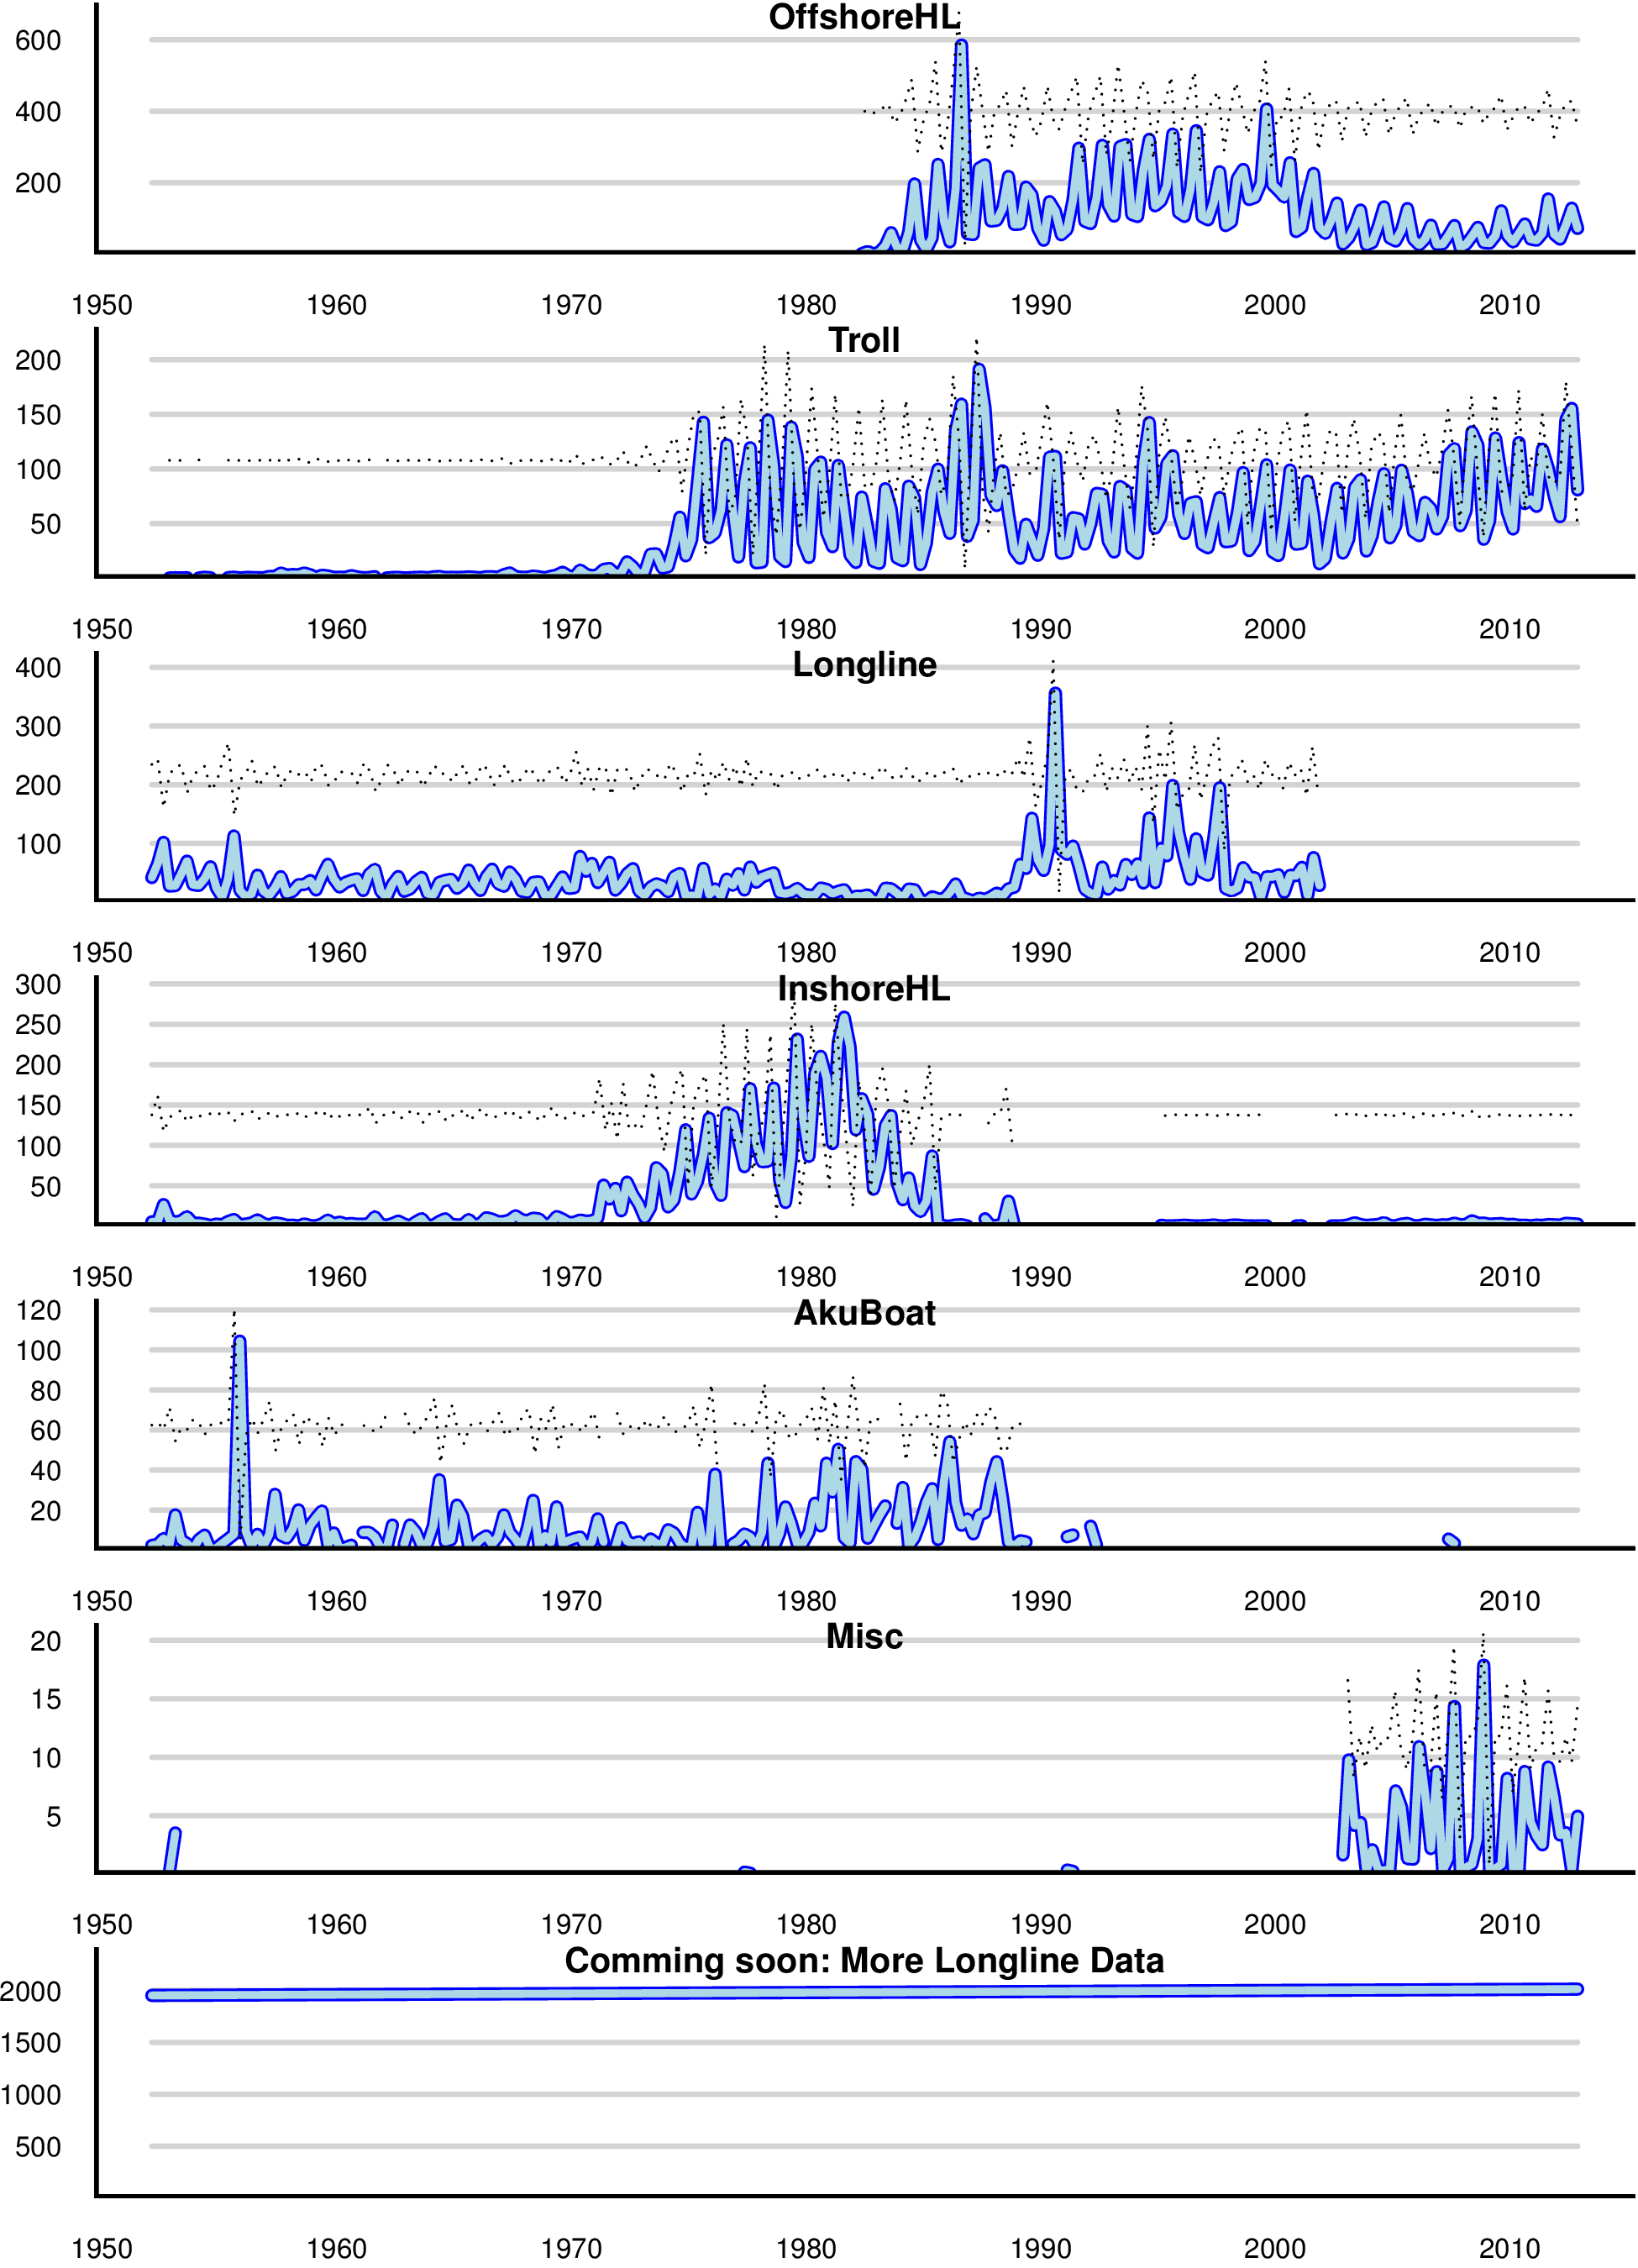
\includegraphics[height=0.9\textheight]{./graphics/catch_history.png}
\caption{\label{fig:catchTS}
Yellowfin catch in metric tonnes by principle fisheries operating in
the Main Hawaiian Islands. The missing data in the bottom panel is
longline data reported on federal logbooks since 1992 which will be
appended to the earlier longline time series.}
\end{center}
\end{figure}

\begin{figure}
\begin{center}
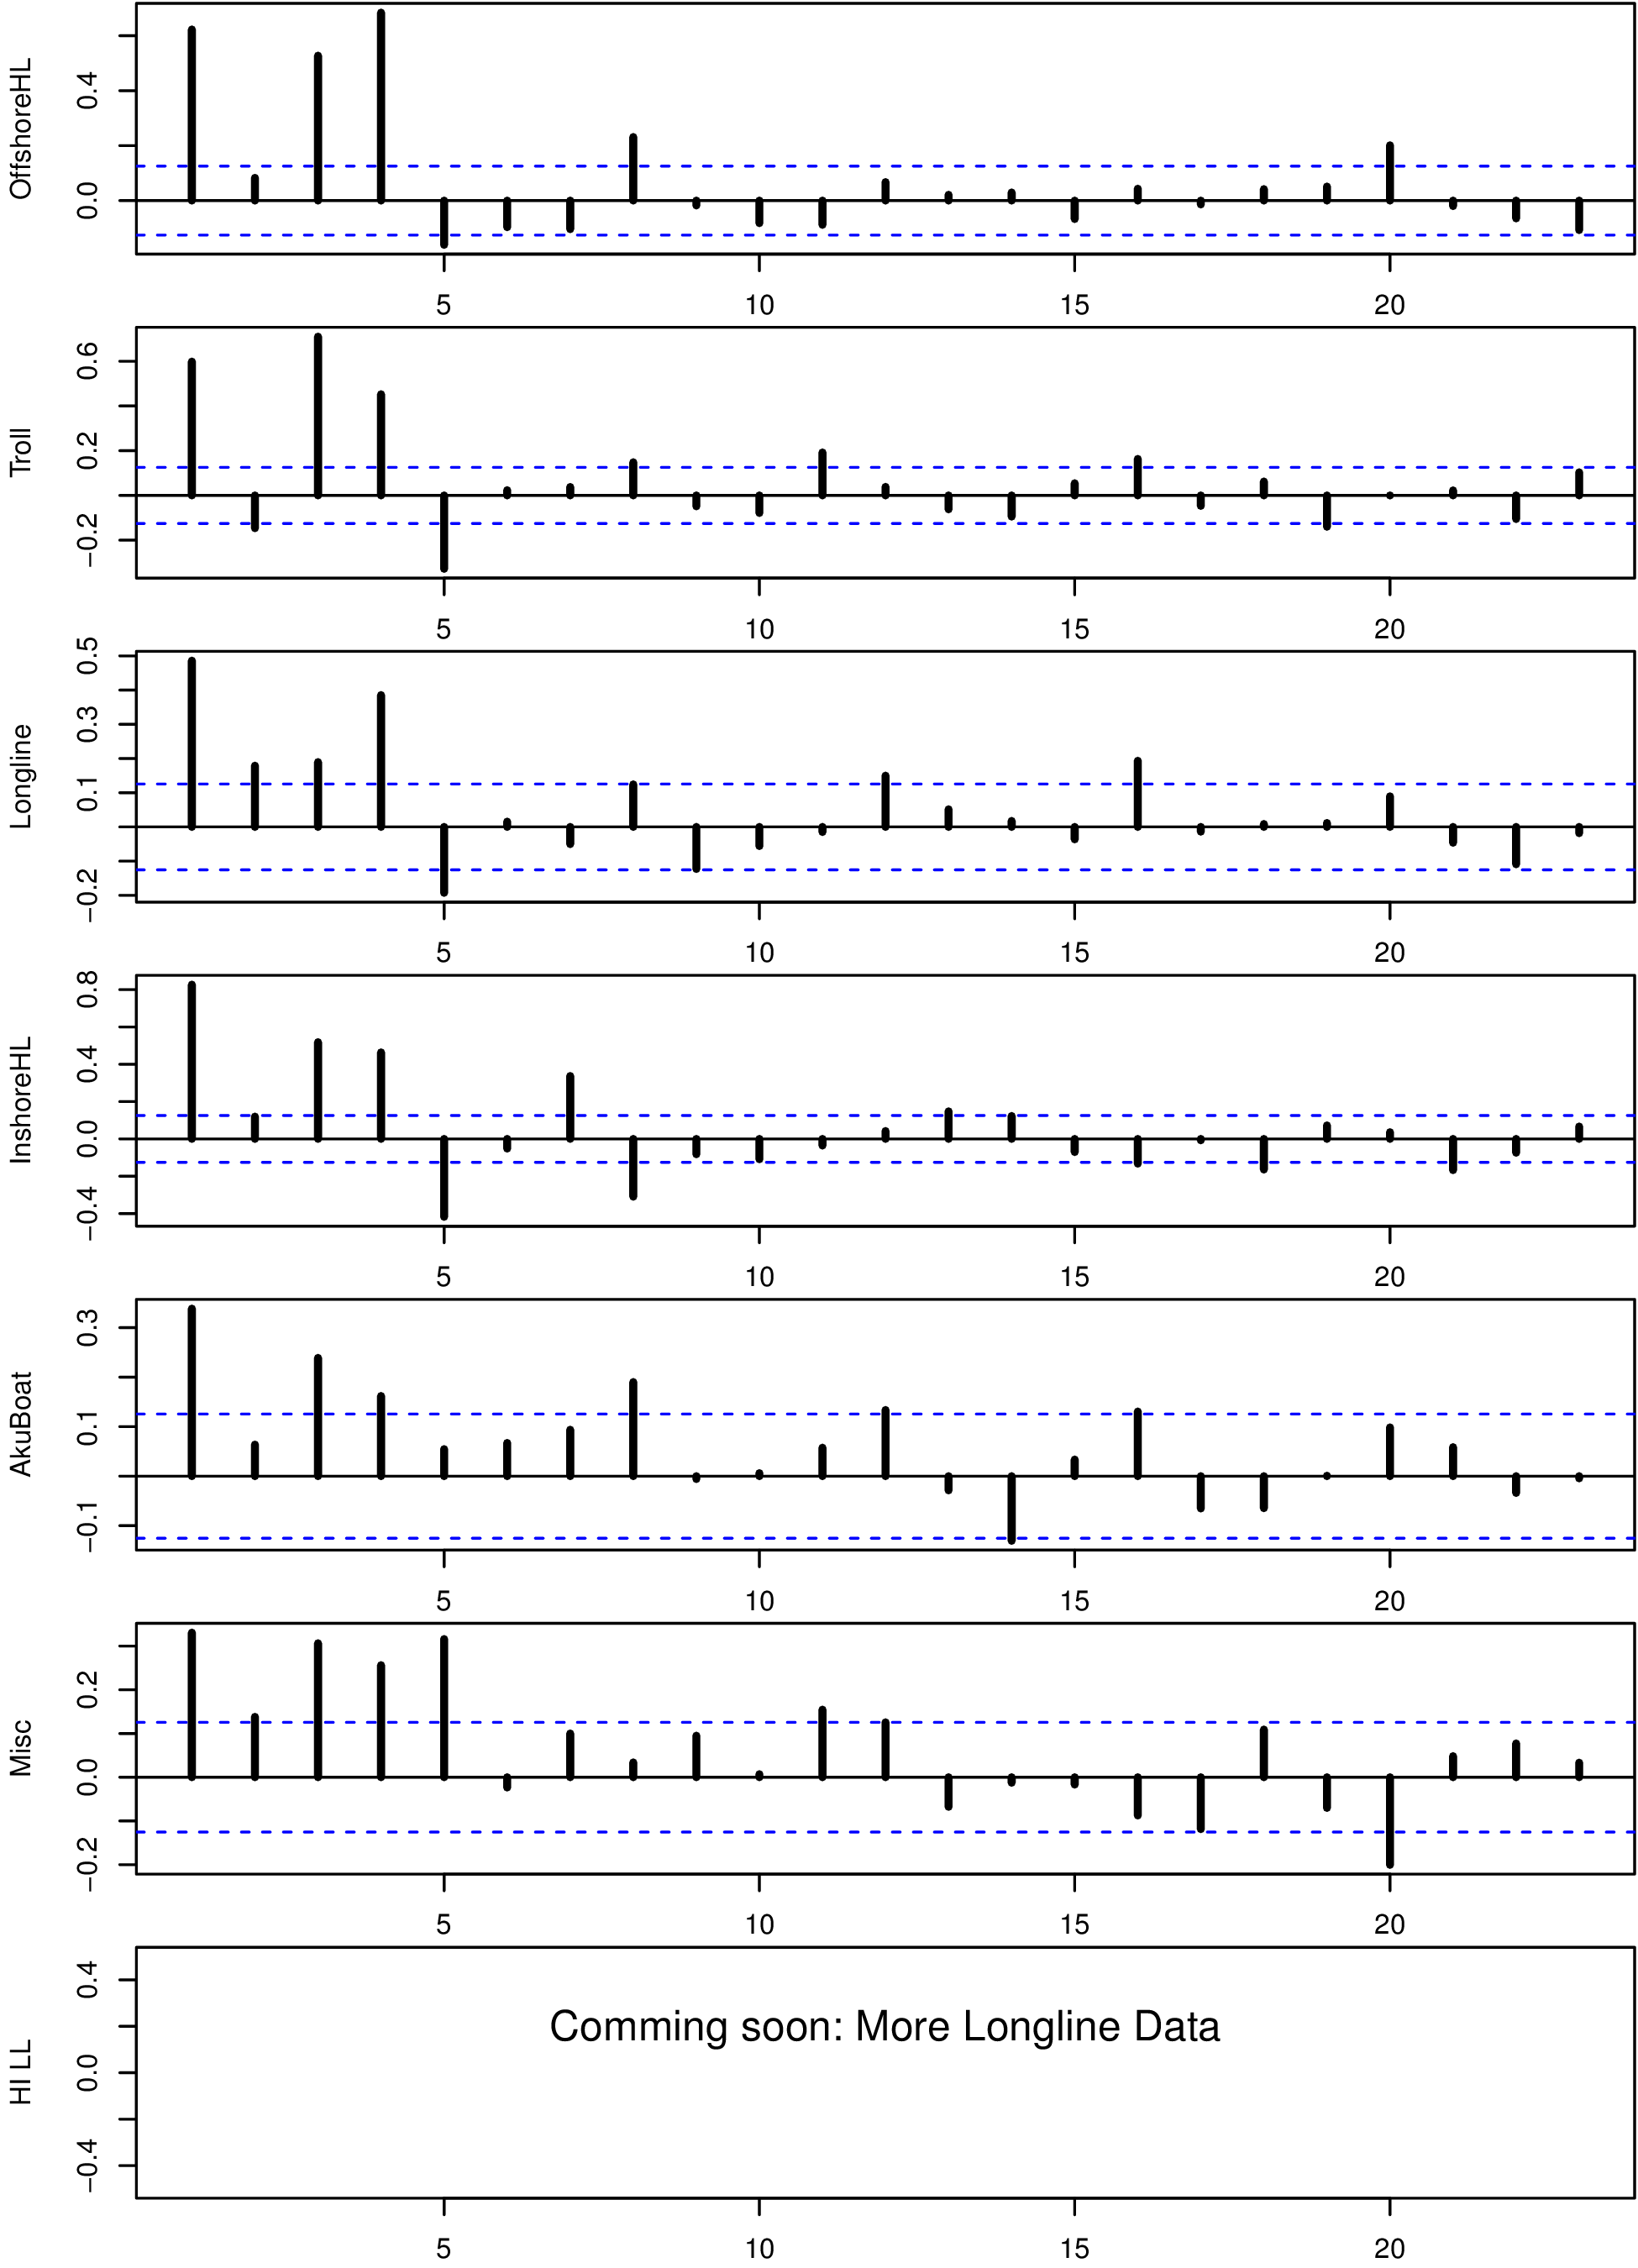
\includegraphics[height=0.9\textheight]{./graphics/partial_acf.png}
\caption{\label{fig:catchPACF}
Partial autocorrelation coefficients of the catch time series. The
dashed blue lines indicate approximate 95\% confidence limits of the
correlations.}
\end{center}
\end{figure}

\begin{figure}
\begin{center}
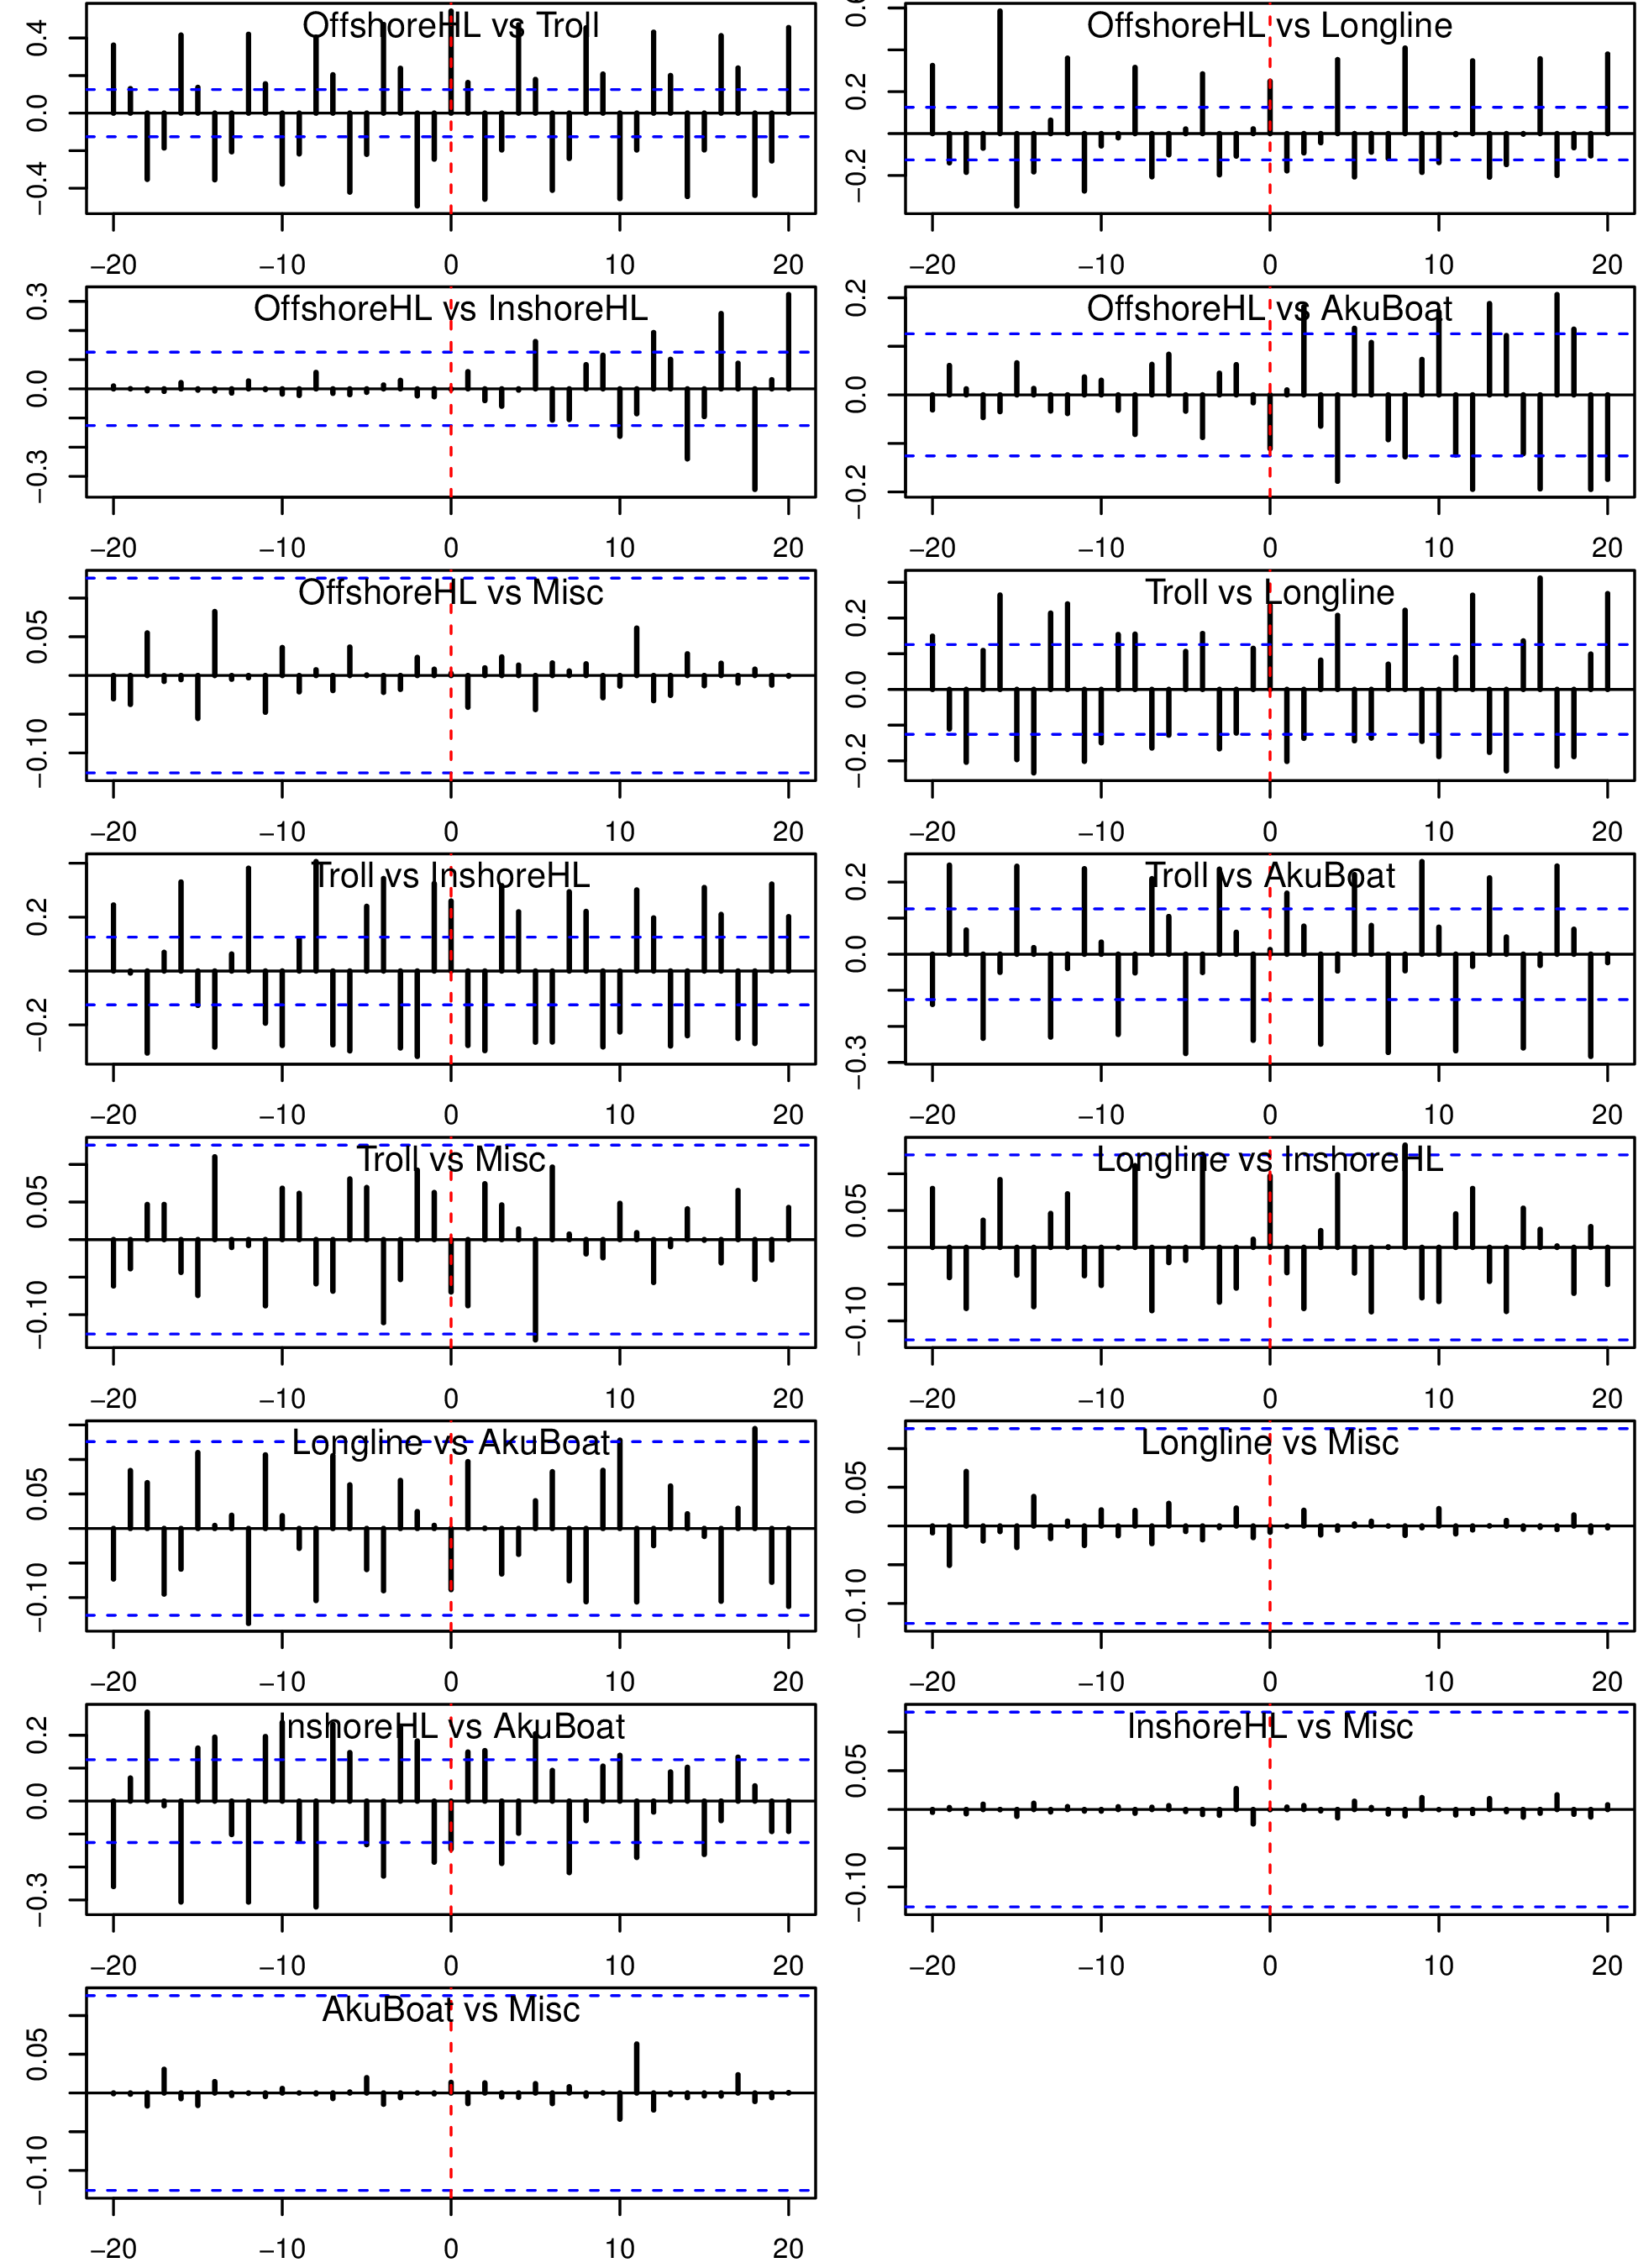
\includegraphics[height=0.9\textheight]{./graphics/ccf.png}
\caption{\label{fig:catchCCF}
Cross correlation coefficients between pairs of the first order
differences of each catch time series at different lags.
The vertical dashed red line emphasize zero lag.
The dashed blue lines indicate approximate 95\% confidence limits of
the correlations.}
\end{center}
\end{figure}

The general modeling approach to be applied will be similar to the
state-space model utilized by Nielsen and Berg (2014). 
State-space models separate variability in the biological
processes in the system (transition model)
from errors in observing features of interest
in the system (observation model). 
The general form of the transition equation is
\begin{equation}
\alpha_t=T(\alpha_{t-1}) + \eta_t
\end{equation}
where the function $T$ embodies the stock dynamics, describing the
development of the state at time $t$ from the state at the previous
time with random process error, $\eta$.
Similarly the general observation equation is
\begin{equation}
x_t = O(\alpha_t) + \varepsilon_t
\end{equation}
where the function $O$ describes the measurement process and with
error $\varepsilon$
Separation if process from measurement offers statistical advantages in
estimating model parameters.

\clearpage
\subsection*{Age-aggregated model: logistic population dynamics (Schaefer Model)}
\help{When this project was initially proposed, I assumed that the
data would not support an age-structured model. Therefore, I began to
think about production model approaches. I'm retaining these ideas in
case the available size data are not sufficient for an multi-gear
age-structured model and because of delays in receiving data.}

Let $\None$ equal the population size of fish originating in region 1
and residing in region 1
and $\Ntwo$ equal the population size of fish originating in region 2
but residing in region 1.
The total population size of fish residing in region 1 is thus
$\Nsum$, and the dynamics of the population in region 1 is represented as
\begin{equation}
\frac{d}{dt}\big(\Nsum\big)=\big(\Nsum\big)\Big[r\Big(1-\frac{\Nsum}{K}\Big) -F - T_{12}\Big] + T_{21}
\label{eqn:logistic}
\end{equation}
where $r$ is the per capita logistic growth rate per year $K$ is the
logistic ``carrying capacity'' measured in the same units as $\None$
and $\Ntwo$, $F$ is the fishing mortality in region 1, and $T_{12}$
is the emigration rate from region 1 to region 2. $T_{21}$
is the annual rate of immigration of fish from region 2 to region 1
measured in the same units as $K$ per year.

Equivalent differential equations could be devised for the dynamics of
fish residing in region 2 (i.e., $\frac{dN_{2,2}}{dt}$ and
$\frac{dN_{1,2}}{dt}$) but 
the dynamics of the fish population in region 2 is external to this
model. $T_{21}$ can be considered to be form of population forcing
from the larger stock in which the MHI population is embedded, perhaps
estimated from other models, such as \MFCL\ or \SD, or perhaps
represented by an
autocorrelated stochastic process. The appearance of
$\Nsum$ in the numerator of the logistic term reflects the assumption
that the population dynamics fish immigrating into region 1 depend on
the population dynamics in region 1. This assumption leads to an
important non-linearity in the model that permits overwhelming of a
local stock by a more numerous immigrant stock as is often characteristics of
mixed-stock fisheries.

The ratio $\frac{\None}{\Nsum}$ is of potential interest, so
equation~\ref{eqn:logistic} needs to be expanded and rearranged
leading to a set of simultaneous differential equation for the
components of the population inhabiting region 1.
\begin{eqnarray}
\frac{d\None}{dt}&=&\None\Big[r\Big(1-\frac{\None}{K}\Big)
-F - T_{12}\Big] - \frac{r}{K}T_{12}\None\Ntwo\nonumber\\
\frac{d\Ntwo}{dt}&=&\Ntwo\Big[r\Big(1-\frac{\Ntwo}{K}\Big)
-F - T_{12}\Big] - \frac{r}{K}T_{12}\None\Ntwo + T_{21}
\label{eqn:coupledschaefer}
\end{eqnarray}
The non-linear term from equation~\ref{eqn:logistic} appears the term
$\None\Ntwo$ in both of the above equations.

The equilibrium of this system can be found by setting
$\frac{d\None}{dt} = 0 = \frac{d\Ntwo}{dt}$. After some simplification
the result is $\frac{T_{21}}{\Ntwo} = 0$ In other words, there is no
equilibrium in this coupled system, other than the degenerate case of
no immigration ($T_{21}=0$) into the MHI. Thus, the notion of using
equilibrium-based reference points such as MSY to manage fisheries for
MHI yellowfin is ill advised.

Equations \ref{eqn:coupledschaefer} are solved by finite difference
approximations using explicit time stepping.
\begin{eqnarray}
\frac{d\None}{dt}\approx\frac{\nextN{\None}-\prevN{\None}}{\Delta t}&=&
\prevN{\None}\Big[r\Big(1-\frac{\prevN{\None}}{K}\Big)
-F - T_{12}\Big]  \nonumber\\
&-& \frac{r}{K}T_{12}\prevN{\None}\prevN{\Ntwo}\nonumber\\
\frac{d\Ntwo}{dt}\approx\frac{\nextN{\Ntwo}-\prevN{\Ntwo}}{\Delta t}&=&
\prevN{\Ntwo}\Big[r\Big(1-\frac{\prevN{\Ntwo}}{K}\Big)
-F - T_{12}\Big]  \nonumber\\
&-& \frac{r}{K}T_{12}\prevN{\None}\prevN{\Ntwo} + T_{21}
\end{eqnarray}
Rearrangement and addition of process error terms ($\eta_{r,t}$)
yields a form suitable for use as the transition equation in a state-space
model.
\begin{eqnarray}
\nextN{\None}=\Bigg[\prevN{\None}&+&{\Delta t}
\prevN{\None}\Big[r\Big(1-\frac{\prevN{\None}}{K}\Big)
-F - T_{12}\Big]\nonumber\\
&-&\frac{r}{K}T_{12}\prevN{\None}\prevN{\Ntwo}
\Bigg]e^{\eta_{1,t}}\nonumber\\
\nextN{\Ntwo}=\Bigg[\prevN{\Ntwo}&+&{\Delta t}
\prevN{\Ntwo}\Big[r\Big(1-\frac{\prevN{\Ntwo}}{K}\Big)
-F - T_{12}\Big]\nonumber\\
&-&\frac{r}{K}T_{12}\prevN{\None}\prevN{\Ntwo}
+T_{21}\Bigg]e^{\eta_{2,t}}
\label{eqn:finitecoupledschaefer}
\end{eqnarray}

\help{
Letting $x_{i,j} = log(N_{i,j})$ then equation
\ref{eqn:coupledschaefer} can be rewritten as
\begin{eqnarray}
\frac{d\log(\None)}{dt} = \frac{dx_{1,1}}{dt}&=&r\Big(1-\frac{\None}{K}\Big)
-F - T_{12} - \frac{r}{K}T_{12}\Ntwo\nonumber\\
\frac{d\log(\Ntwo)}{dt} = \frac{dx_{1,2}}{dt}&=&r\Big(1-\frac{\Ntwo}{K}\Big)
-F - T_{12} - \frac{r}{K}T_{12}\None + T_{21}/\Ntwo
\label{eqn:coupledlogschaefer}
\end{eqnarray}
and the finite difference equivalent of
\ref{eqn:finitecoupledschaefer} becomes
\begin{eqnarray}
x_{1,1,t} &=& x_{1,1,t-\Delta t} +r\Delta t\Big(1-\frac{\None_{t-\Delta t}}{K}\Big)
-F - T_{12} - \frac{r}{K}T_{12}\Ntwo_{t-\Delta t}+\eta_{1,t}\nonumber\\
x_{1,2,t} &=& x_{1,2,t-\Delta t} +r\Delta t\Big(1-\frac{\Ntwo_{t-\Delta t}}{K}\Big)
-F - T_{12} - \frac{r}{K}T_{12}\None_{t-\Delta t} + T_{21}/\Ntwo_{t-\Delta t}+\eta_{2,t}
\label{eqn:finitecoupledlogschaefer}
\end{eqnarray}
This parameterization may be simple, but using my simulation, I
don't get the same answer as I get from
\ref{eqn:finitecoupledschaefer}. Perhaps I have made a math error of
did not implement it correctly in R.

} %\help{


\subsection*{Age-aggregated model: (Pella-Tomlinson Model)}
\help{Probably not worth the effort.}

%\clearpage
\subsection*{Age structured model}
\newcommand{\NNone}[2]{N_{1,#1,#2}}
\newcommand{\NNtwo}[2]{N_{2,#1,#2}}
The issue of regulating MHI YFT fisheries by imposing minimum size
limits on some components of the fishery has been raised yet again.
Size- or age-structured models are obviously required to address catch-at-size
issues. The following set of equations are a potential formulation
of the transition equation in an age-structured state-space model 
and are based on the
state-space stock assessment model of Nielsen and Bert (2014). 
Let $N_{r,a,t}$ represent the fish living
in the MHI but originating in in region $r; r = 1,2$ of age $a; a =
1, 2, \ldots, A$ in time interval $t$.
\begin{eqnarray}
\log\NNone{1}{t}&=&\log\Big(R\big(\sum_a{p_{a,t-1}(\NNone{a}{t-1}+\NNtwo{a}{t-1})}\big)\Big)+\eta_{1,1,t}\\
\log\NNtwo{1}{t}&=&\log T_{2,1,1,t}+\eta_{2,1,t}\\
\nonumber\\
\log\NNone{a}{t}&=&\log\NNone{a-1}{t-1}-Z_{a-1,t-1}+\eta_{1,a,t};\qquad 1<a<A \\
\log\NNtwo{a}{t}&=&\log\NNtwo{a-1}{t-1}-Z_{a-1,t-1}+\log T_{2,1,a,t}+\eta_{2,a,t}\\
\nonumber\\
\log\NNone{A}{t}&=&\log\NNone{A-1}{t-1}-Z_{A-1,t-1}+\log\NNone{A}{t-1}-Z_{A,t-1}+\eta_{1,A,t}\\
\log\NNtwo{A}{t}&=&\log\NNtwo{A-1}{t-1}-Z_{A-1,t-1}+\log\NNtwo{A}{t-1}-Z_{A,t-1}+\log T_{2,1,A,t}+\eta_{2,A,t} 
\end{eqnarray}
where $Z_{a,t} = \sum_gF_{g,a,t}+M_{a}+T_{1,2}$ is a positive quantity
representing the total mortality at fish of age $a$ in time interval
$t$,
$M_{a}$ is the natural mortality at age $a$, assumed to be constant
over time, and
$F_{g,a,y}$ is the fishing mortality exerted by gear $g$, on fish of
age $a$ during time period $t$. 

\help{Is it appropriate to use different process error time series 
($\eta_{1,t}$ and $\eta_{2,t}$) for the two
segments of the population under the assumption of identical population
dynamics for both segments?}

The immigration term, $T_{2,1,a,t}$, is the biomass of fish of age
$a$ immigrating from region 2 to region 1 during time period $t$.
Immigration is assumed to be proportional to the biomass of yellowfin
adjacent to the MHI as might be estimated by \MFCL\ or \SD. Thus
\begin{equation}
T_{2,1,a,t} = T_{2,1}^\prime \cdot \widehat{B_{2,a,t}}
\end{equation}

Fishing mortality is often
represented in stock assessment models as the product of several
parameters and variables, for example, 
catchability coefficient, gear selectivity, and fishing
effort. The parameters of this relationship are usually confounded and
difficult to estimate. In the case of MHI yellowfin
fishery, effort estimates are known to be inconsistent, and fishing
practices have changed over time often
requiring {\it ad hoc}
adjustments to catchability and gear selectivity. Eliminating 
fishing effort would simply the model somewhat.

Fishing mortality is assumed to to follow a random walk with
multivariate normal increments, with major
seasonally (by quarter) variation, and to
depend on gear selectivity.
\begin{equation}
\log F_{g,a,t} = \log F_{g,a,t-1}+\alpha_{g,Q(t)}+\beta_{g,Y(t)}
+S_{g,a,t}+\varepsilon_t
\label{eqn:fmort}
\end{equation}
$\alpha$ is a vector of quarterly deviations from the mean
fishing mortality that sum to zero.
$\beta$ is a vector of autocorrelated annual deviations from the mean
that reflect secular trends in fishing mortality.
$S_{g,a,t}$ represents the selectivity of gear $g$ on age class $a$
fish during time period $t$.


%Independent estimates of Pacific YFT natural morality at age are
%available from \MFCL\ (Davies,et al 2014), and estimates of MHI YFT
%natural mortality by size class
%are available from Adam (et al 2003).
%$T_{1,2}$ is the instantaneous transfer rate of
%fish out of the MHI assumed to be independent of age of fish.
%$T_{2,1,a,y}$ is the total rate of transfer of age
%$a$ fish into the MHI in year $y$ which could be parameterized as a simple
%proportion of the numbers at age estimated from \MFCL.

%The fisheries data for the MHI do not include catch at age, but rather
%catch at weight or catch at length.
%\begin{equation}
%q_{l,a,t} =
%\frac{\omega}{\sqrt{2\pi}\sigma_a}e^{\frac{-(x_l-\mu_a)^2}{2\sigma_a}}
%\end{equation}

The observation model predicting the yield or catch in the MHI
under 
this model would be
\begin{equation}
C_{g,a,t} =
\frac{F_{g,a,t}}{Z_{g,a,t}}\Big(1-e^{Z_{g,a,t}}\Big)\Big(\NNone{a}{t}+\NNtwo{a}{t}\Big)e^{\varepsilon_{g,a,t}}
\end{equation}
using the standard Baranov approximation.

\singlespacing
\section*{References}
{\parindent=0cm \small
\everypar={\hangindent=2em \hangafter=1}\par
\doublespacing
Adam, M. S., J. Sibert, D. Itano and K. Holland. 2003. Dynamics of
bigeye (Thunnus obesus) and yellowfin tuna (T. albacares) in Hawaii's
pelagic fishery: analysis of tagging data with a bulk transfer model
incorporating size specific attrition. Fishery Bulletin 101(2):
215-228.

Davies, N., S. Harley, J. Hampton, S. McKechnie. 2014. Stock
assessment of yellowfin tuna in the western and central pacific ocean.
WCPFC-SC10-2014/SA-WP-04.

Itano, D., K. Holland. 2000.  Movement and vulnerability of bigeye
(Thunnus obesus) and yellowfin tuna (Thunnus albacares) in relation to
FADs and natural aggregation points.Aquat. Living Resour. 13: 213-223.

Kleiber, P., J. Hampton, N. Davies, S. Hoyle, D. Fournier. 2014.
MULTIFAN-CL User’s Guide

Nielsen, A. and C. Berg. 2014. Estimation of time-varying selectivity
in stock assessments usingstate-space models. Fisheries Research
158:96-101.

Wells, D., J. Rooker, D. Itano. 2012.  Nursery origin of yellowfin
tuna in the Hawaiian Islands. Mar. Ecol. Prog. Ser. 461:187-196. 
\par}

%%%%%%%% figures begin here %%%%%%%%%%%%%%%%%%%%%%
\end{document}
